% !TeX root = main.tex

\chapter{随机事件及其概率}
\thispagestyle{plain}

\section{随机事件}

\subsection{随机试验}

在一定条件下必然出现的现象叫做\textbf{必然现象}.在相同的条件下,可能出现不同的结果,而在试验或观测之前不能预知确切结果的现象叫做\textbf{随机现象}.

随机现象具有随机性和统计规律性.

\begin{itemize}
    \item 随机性:对随机现象进行观测时,不能预先确定其结果.
    \item 统计规律性:对随机现象进行大量重复观测后,其结果往往会表现出某种规律性.
\end{itemize}

为了研究和揭示随机现象的统计规律性,需要对随机现象进行大量重复的观察、测量或试验,统称为试验.

如果试验具有以下特点:
\begin{enumerate}
    \item 可重复性:试验可以在相同条件下重复进行多次,甚至进行无限次;
    \item 可观测性:每次试验的所有可能结果都是明确的、可以观测的,并且试验的可能结果有两个或两个以上;
    \item 随机性:每次试验出现的结果是不确定的,在试验之前无法预先确定究竟会出现哪一个结果,
\end{enumerate}
则称之为\textbf{随机试验}(random experiment),简称为\textbf{试验}(experiment).

通常用字母 $E$ 表示一个随机试验. 随机试验 $E$ 的基本结果称为\textbf{样本点}(sample point),用 $\omega$ 表示.随机试验 $E$ 的所有基本结果的集合称为\textbf{样本空间}(sample space),用 $\varOmega = \{ \omega \}$ 表示.

\begin{note}
    \begin{enumerate}
        \item 样本空间中的元素可以是数,也可以不是数.
        \item 随机现象的样本空间至少有2个样本点.只有1个样本点的样本空间对应必然现象.
        \item 根据样本点个数,可以将样本空间分为有限与无限两类.在一个样本空间中,如果只有有限个样本点,则称它为\textbf{有限样本空间};如果有无限个样本点,则称它为\textbf{无限样本空间}.
        \item 另一种分类方式:样本点个数为有限个或可列个时,称为\textbf{离散样本空间};样本点个数为不可列无限个时,称为\textbf{连续样本空间}.
    \end{enumerate}
\end{note}

\subsection{随机事件的概念}

随机试验 $E$ 的样本空间 $\varOmega = \{ \omega \}$ 的子集称为随机试验 $E$ 的\textbf{随机事件}(random event),简称为\textbf{事件}(event),用大写字母 $A,B,C$ 等表示.

设 $A \subseteq \varOmega$,如果试验结果 $\omega \in A$,则称在这次试验中事件 $A$ 发生;如果 $\omega \notin A$,则称事件 $A$ 不发生.

由一个样本点 $\omega$ 组成的事件称为\textbf{基本事件}(elementary event).

$\varOmega$ 本身也是 $\varOmega$ 的子集,在每次试验中必然发生,称为\textbf{必然事件}(certain event).

空集 $\text{\O}$ 也是 $\varOmega$ 的子集,在试验中不可能发生,称为\textbf{不可能事件}(impossible event).

必然事件和不可能事件统称为\textbf{确定事件}.

\subsection{随机事件的关系}

\subsubsection{事件的包含}

如果当事件 $A$ 发生时事件 $B$ 一定发生,则称事件 $B$ \textbf{包含}事件 $A$,或称事件 $A$ 包含于事件 $B$,记作 $A \subseteq B$.

\begin{property}
    \indent 对于任意事件 $A$,有 $\text{\O} \subseteq A \subseteq \varOmega$.
\end{property}

\begin{property}
    \indent 如果 $A \subseteq B, B \subseteq C$,则 $A\subseteq C$.
\end{property}

\subsubsection{事件的相等}

如果事件 $A$ 与 $B$ 相互包含,即 $A \subseteq B$ 且 $B \subseteq A$,则称事件 $A$ 与事件 $B$ \textbf{相等},记作 $A=B$.

\subsubsection{事件的互斥}

如果事件 $A$ 和事件 $B$ 在同一次试验中不能同时发生,则称事件 $A$ 与事件 $B$ \textbf{互斥}(mutually exclusive),或称事件 $A$ 与事件 $B$ \textbf{互不相容}.

任意两个基本事件一定互斥.

不可能事件 $\text{\O}$ 与任意事件互斥.

\subsubsection{事件的互逆}

如果在每一次试验中事件 $A$ 和事件 $B$ 必有一个且仅有一个发生,则称事件 $A$ 与事件 $B$ 是\textbf{互逆}的或\textbf{对立}的,称事件 $A$ 与事件 $B$ 互为\textbf{逆事件}或\textbf{对立事件}(complementary events),记作 $\overline{A}=B$,或 $\overline{B}=A$.

对立事件一定互斥. 反之,互斥的事件不一定对立.

\begin{property}
    \indent 对于任意事件 $A$,有 $\overline{\overline{A}}=A$.
\end{property}

\subsection{随机事件的运算}

\subsubsection{事件的并}

如果事件 $A$ 和事件 $B$ 至少有一个发生,则这样的一个事件称为事件 $A$ 与事件 $B$ 的\textbf{并事件}(union event)或\textbf{和事件},记作 $A \cup B$.
$$
A \cup B = \{ \omega \mid \omega \in A \;\text{或}\; \omega \in B \}
$$

事件 $A$ 和事件 $B$ 作为样本空间 $\varOmega$ 的子集,并事件 $A \cup B$ 就是集合 $A$ 与 $B$ 的并集.

\begin{property}
    \indent 对于任意事件 $A$ 与 $B$,有:
    \begin{enumerate}
        \item $A \cup A = A$.
        \item $A \cup \text{\O} = A$.
        \item $A \cup B = B \cup A$.
        \item $A \cup \overline{A} = \varOmega$.
        \item $A \subseteq A \cup B, B \subseteq A \cup B$.
        \item 如果 $A \subseteq B$,则有 $A \cup B=B$.
    \end{enumerate}
\end{property}

事件的并可以推广到多个事件的情形.对于事件 $A_1,A_2,\cdots,A_n,\cdots$, $\displaystyle\bigcup_{i=1}^n A_i$ 称为有限并, $\displaystyle\bigcup_{i=1}^\infty A_i$ 称为可列并.

\subsubsection{事件的交}

如果事件 $A$ 和事件 $B$ 同时发生,则这样的一个事件称为事件 $A$ 与事件 $B$ 的\textbf{交事件}(intersection event)或\textbf{积事件},记作 $A \cap B$ 或 $AB$.
$$
A \cap B = \{ \omega \mid \omega \in A \;\text{且}\; \omega \in B \}
$$

事件 $A$ 和事件 $B$ 作为样本空间 $\varOmega$ 的子集,交事件 $A \cap B$ 就是集合 $A$ 与 $B$ 的交集.

\begin{property}
    \indent 对于任意事件 $A$ 与 $B$,有:
    \begin{enumerate}
        \item $A \cap A = A$.
        \item $A \cap \text{\O} = \text{\O}$.
        \item $A \cap B = B \cap A$.
        \item $A \cap \overline{A} = \text{\O}$.
        \item $A \cap B \subseteq A, A \cap B \subseteq B$.
        \item 如果 $A \subseteq B$,则有 $A \cap B = A$.
        \item 如果 $A$ 与 $B$ 互斥,则有 $A \cap B = \text{\O}$.
    \end{enumerate}
\end{property}

事件的交可以推广到多个事件的情形.对于事件 $A_1,A_2,\cdots,A_n,\cdots$, $\displaystyle\bigcap_{i=1}^n A_i$ 称为有限交, $\displaystyle\bigcap_{i=1}^\infty A_i$ 称为可列交.

\begin{conclusion}
    \indent 事件 $A$ 与 $B$ 对立的充分必要条件是: $A \cap B = \text{\O}$,且 $A \cup B = \varOmega$.
\end{conclusion}

\subsubsection{事件的差}

如果事件 $A$ 发生而事件 $B$ 不发生,则这样的一个事件称为事件 $A$ 与事件 $B$ 的\textbf{差事件}(difference event),记作 $A-B$.
$$
A - B = \{ \omega \mid \omega \in A \;\text{且}\; \omega \notin B \}
$$

\begin{property}
    \indent 对于任意事件 $A$ 与 $B$,有:
    \begin{enumerate}
        \item $A - A = \text{\O}$
        \item $A - \text{\O} = A$
        \item $\text{\O} - A = \text{\O}$
        \item $\varOmega - A = \overline{A}$
        \item $A - \varOmega = \text{\O}$
        \item $A - B = A - AB = A \overline{B}$
        \item $A \cup B = A \cup (B-A) = A \cup (B-AB)$
        \item $A \cup B = B \cup (A-B) = B \cup (A-AB)$
        \item $A-B, AB, B-A$ 两两互斥,且 \\
        (1) $A \cup B = (A-B) \cup AB \cup (B-A)$ \\
        (2) $A = (A-B) \cup AB$ \\
        (3) $B = (B-A) \cup AB$
    \end{enumerate}
\end{property}

\subsubsection{随机事件的运算性质}

\begin{property}
    \begin{enumerate}
        \item 交换律
        $$
        \begin{gathered}
            A \cup B = B \cup A \\
            AB=BA
        \end{gathered}
        $$
        \item 结合律
        $$
        \begin{gathered}
            (A \cup B) \cup C = A \cup (B \cup C) \\
            (AB)C=A(BC)
        \end{gathered}
        $$
        \item 分配律
        $$
        \begin{gathered}
            A(B \cup C) = (AB) \cup (AC) \\
            A \cup (BC) = (A \cup B)(A \cup C)
        \end{gathered}
        $$
        \item 对偶律(德摩根公式)
        $$
        \begin{gathered}
            \overline{A \cup B} = \overline{A} \cap \overline{B} \\
            \overline{A \cap B} = \overline{A} \cup \overline{B}
        \end{gathered}
        $$
    \end{enumerate}
\end{property}

对偶律的证明如下.

\begin{proof}
    设样本点 $\omega \in \overline{A \cup B}$,则 $\omega \notin A \cup B$,即 $\omega \notin A$ 和 $\omega \notin B$ 同时成立,所以 $\omega \in \overline{A}$ 和 $\omega \in \overline{B}$ 同时成立,于是有 $\omega \in \overline{A} \cap \overline{B}$,这说明
    $$
    \overline{A \cup B} \subseteq \overline{A} \cap \overline{B}
    $$
    反之,设 $\omega \in \overline{A} \cap \overline{B}$,即 $\omega \in \overline{A}$ 和 $\omega \in \overline{B}$ 同时成立,从而有 $\omega \notin A$ 和 $\omega \notin B$ 同时成立,这意味着 $\omega$ 不属于 $A$ 与 $B$ 中的任意一个,即 $\omega \notin A \cup B$,也就是 $\omega \in \overline{A \cup B}$,这说明
    $$
    \overline{A} \cap \overline{B} \subseteq \overline{A \cup B}
    $$
    综上可得
    $$
    \overline{A \cup B} = \overline{A} \cap \overline{B}
    $$

    同理,设样本点 $\omega \in \overline{A \cap B}$,则 $\omega \notin A \cap B$,即 $\omega \in A$ 和 $\omega \in B$ 不能同时成立,所以 $\omega \in \overline{A}$ 和 $\omega \in \overline{B}$ 至少有一个成立,于是有 $\omega \in \overline{A} \cup \overline{B}$,这说明
    $$
    \overline{A \cap B} \subseteq \overline{A} \cup \overline{B}
    $$
    反之,设 $\omega \in \overline{A} \cup \overline{B}$,则 $\omega \in \overline{A}$ 和 $\omega \in \overline{B}$ 至少有一个成立,即 $\omega \in A$ 和 $\omega \in B$ 不能同时成立,所以 $\omega \notin A \cap B$,即 $\omega \in \overline{A \cap B}$,这说明
    $$
    \overline{A} \cup \overline{B} \subseteq \overline{A \cap B}
    $$
    综上可得
    $$
    \overline{A \cap B} = \overline{A} \cup \overline{B}
    $$
\end{proof}

对于多个及可列个随机事件,以上的运算性质也成立.例如,在多个及可列个事件的情况下,对偶律可以推广为
$$
\overline{\bigcup_{i=1}^n A_i} = \bigcap_{i=1}^n \overline{A_i}, \quad \overline{\bigcup_{i=1}^{+\infty} A_i} = \bigcap_{i=1}^{+\infty} \overline{A_i},\quad \overline{\bigcap_{i=1}^n A_i} = \bigcup_{i=1}^n \overline{A_i}, \quad \overline{\bigcap_{i=1}^{+\infty} A_i} = \bigcup_{i=1}^{+\infty} \overline{A_i}
$$

\subsection{事件域}

\begin{definition}[][][def:事件域]
    \indent 设 $\varOmega$ 为样本空间, $\mathcal{F}$ 为 $\varOmega$ 的某些子集组成的集合类.如果 $\mathcal{F}$ 满足:
    \begin{enumerate}
        \item $\varOmega \in \mathcal{F}$;
        \item 若 $A \in \mathcal{F}$,则 $\overline{A} \in \mathcal{F}$;
        \item 若 $A_i \in \mathcal{F}, \, i=1,2,\cdots$,则 $\displaystyle\bigcup_{i=1}^\infty A_i \in \mathcal{F}$,
    \end{enumerate}
    则称 $\mathcal{F}$ 为一个\textbf{事件域}(event domain),也称为 $\sigma$ \textbf{域}或 $\sigma$ \textbf{代数}.将 $(\varOmega, \mathcal{F})$ 称为\textbf{可测空间}(measurable space).
\end{definition}

在可测空间上才可定义概率,这时 $\mathcal{F}$ 中都是有概率可言的事件.

\begin{note}
    \indent 事件域就是样本空间中某些子集及其运算结果组成的集合类.对于离散样本空间,它的所有子集就构成了事件域.而对连续样本空间,存在无法测量长度的子集,这样的集合称为\textbf{不可测集}.如果将不可测集也看成事件,那么这样的事件将没有概率可言.因此,没有必要将连续样本空间的所有子集都看做事件,只需将可度量的子集(称为\textbf{可测集})看做事件即可.

    \indent 事件域包含样本空间的所有可测子集,这些子集可以看做有概率可言的事件.事件之间可以进行运算,并且运算结果仍然是事件,因此事件域要对事件的各种运算具有封闭性.

    \indent 在事件的各种运算中,并与对立是最基本的运算,因为:
    \begin{itemize}
        \item 交运算可通过并与对立来实现($A \cap B = \overline{\overline{A} \cup \overline{B}}$).
        \item 差运算可通过对立与交来实现($A-B = A \overline{B}$).
    \end{itemize}
    所以,只需事件域对并运算和对立运算封闭,这就是定义 \ref{def:事件域} 的来源.
\end{note}

\begin{property}
    \indent 可测空间 $(\varOmega, \mathcal{F})$ 的性质:
    \begin{enumerate}
        \item $\text{\O} \in \mathcal{F}$.
        \item 若 $A_i \in \mathcal{F}, \, i=1,2,\cdots,n$,则 $\displaystyle\bigcup_{i=1}^n A_i \in \mathcal{F}$.
        \item 若 $A_i \in \mathcal{F}, \, i=1,2,\cdots$,则 $\displaystyle\bigcap_{i=1}^{\infty} A_i \in \mathcal{F}$.
        \item 若 $A_i \in \mathcal{F}, \, i=1,2,\cdots,n$,则 $\displaystyle\bigcap_{i=1}^n A_i \in \mathcal{F}$.
        \item 若 $A,B \in \mathcal{F}$,则 $A-B \in \mathcal{F}$.
    \end{enumerate}
\end{property}

\begin{proof}
    (1)由定义 \ref{def:事件域} 可知, $\varOmega \in \mathcal{F}$,进而有
    $$
    \overline{\varOmega} = \text{\O} \in \mathcal{F}
    $$

    (2)令 $A_{i} = \text{\O},\; i = n+1, n+2, \cdots$,则由定义 \ref{def:事件域} 可得
    $$
    \bigcup_{i=1}^{\infty} A_i = \bigcup_{i=1}^{n} A_i \in \mathcal{F}
    $$

    (3)若 $A_i \in \mathcal{F}$,则 $\overline{A_i} \in \mathcal{F}$,因此
    $$
    \bigcup_{i=1}^{\infty} \overline{A_i} = \overline{\bigcap_{i=1}^{\infty} A_i} \in \mathcal{F}
    $$
    进而有
    $$
    \bigcap_{i=1}^{\infty} A_i \in \mathcal{F}
    $$

    (4)若 $A_i \in \mathcal{F}$,则 $\overline{A_i} \in \mathcal{F}$,因此
    $$
    \bigcup_{i=1}^{n} \overline{A_i} = \overline{\bigcap_{i=1}^{n} A_i} \in \mathcal{F}
    $$
    进而有
    $$
    \bigcap_{i=1}^{n} A_i \in \mathcal{F}
    $$

    (5)因为 $B \in \mathcal{F}$,所以 $\overline{B} \in \mathcal{F}$,进而有
    $$
    A-B = A \overline{B} \in \mathcal{F}
    $$
\end{proof}

若样本空间含有 $n$ 个样本点,则其事件域 $\mathcal{F}$ 是由空集 $\text{\O}$、$n$ 个单元素集、$\mathrm{C}_n^2$ 个双元素集、$\mathrm{C}_n^3$ 个三元素集……和 $\varOmega$ 组成的集合类,此时 $\mathcal{F}$ 中共有 $\mathrm{C}_n^0 + \mathrm{C}_n^1 + \mathrm{C}_n^2 + \cdots + \mathrm{C}_n^n = 2^n$ 个事件.

若样本空间含有可列个样本点,则其事件域 $\mathcal{F}$ 是由空集 $\text{\O}$、可列个单元素集、可列个双元素集……可列个 $n$ 元素集……和 $\varOmega$ 组成的集合类,此时 $\mathcal{F}$ 由可列个事件组成.

如果样本空间为全体实数,即 $\varOmega = \mathbf{R}$,此时事件域 $\mathcal{F}$ 中的元素无法一一列出,而是由一个基本集合类逐步扩展形成,具体操作如下:
\begin{enumerate}
    \item 取基本集合类 $\mathcal{P}$ 为``全体半直线组成的类",即
    $$
    \mathcal{P} = \{ (-\infty, x) \mid -\infty < x < +\infty \}
    $$
    \item 把有限的左闭右开区间扩展进来
    $$
    [a,b) = (-\infty,b) - (-\infty,a), \, a,b \in \mathbf{R}
    $$
    \item 把闭区间、单点集、左开右闭区间、开区间扩展进来
    $$
    \begin{aligned}
        & [a,b] = \bigcap_{i=1}^{\infty} \Big[ a, b + \dfrac{1}{i} \Big) \\
        & \{ b \} = [a,b] - [a,b) \\
        & (a,b] = [a,b] - \{ a \} \\
        & (a,b) = [a,b) - \{ a \}
    \end{aligned}
    $$
    \item 最后用(有限个或可列个)并运算和交运算把实数集中一切有限集、可列集、开集、闭集都扩展进来.
\end{enumerate}
经过上述几步扩展所得集合的全体就是事件域 $\mathcal{F}$,这样的事件域 $\mathcal{F}$ 又称为\textbf{博雷尔事件域},域中的每个元素称为\textbf{博雷尔集}(Borel set).

\begin{definition}
    \indent 对样本空间 $\varOmega$,如果事件 $A_1,A_2,\cdots,A_n$ 互斥,且 $\displaystyle\bigcup_{i=1}^n A_i=\varOmega$,则称 $A_1,A_2,\cdots,A_n$ 为样本空间 $\varOmega$ 的一个\textbf{分割}或\textbf{完全事件组}(collectively exhaustive events).
\end{definition}

若 $A = \{ A_1,A_2,\cdots,A_n \}$ 为样本空间 $\varOmega$ 的一个分割,由分割 $A$ 产生的事件域记作 $\sigma(A)$,则 $\sigma(A)$ 中含有 $2^n$ 个不同的事件.利用分割可以将事件域简化,从而简化所研究的问题.

\section{随机事件的概率}

\subsection{频率}

\begin{definition}
    \indent 设在相同的条件下进行的 $n$ 次试验中,事件 $A$ 发生了 $n_A$ 次,则称 $n_A$ 为事件 $A$ 发生的\textbf{频数}(frequency),称比值 $\dfrac{n_A}{n}$ 为事件 $A$ 发生的\textbf{频率}(relative frequency),记作 $f_n(A)$,即
    $$
    f_n(A)=\dfrac{n_A}{n}
    $$
\end{definition}

事件 $A$ 发生的频率反映了事件 $A$ 在 $n$ 次试验中发生的频繁程度.频率越大,表明事件 $A$ 的发生越频繁,从而可知事件 $A$ 在一次试验中发生的可能性越大.

\begin{property}[][频率的基本性质]
    \begin{enumerate}
        \item \textbf{非负性}:对于任意事件 $A$,有 $f_n(A) \geqslant 0$.
        \item \textbf{规范性}:对于必然事件 $\varOmega$,有 $f_n(\varOmega)=1$.
        \item \textbf{有限可加性}:对于两两互斥的事件 $A_1,A_2,\cdots,A_m$,有
        $$
        f_n \left(\bigcup_{i=1}^m A_i \right) = \sum_{i=1}^m f_n(A_i)
        $$
    \end{enumerate}
\end{property}

频率 $f_n(A)$ 依赖于试验次数 $n$ 及每次试验的结果.当 $n$ 较小时,频率的波动性一般较大.当 $n$ 增大时,频率 $f_n(A)$ 呈现出稳定性,逐渐稳定于某一常数 $p$,用这一常数表示事件 $A$ 发生的可能性大小,称为事件 $A$ 的概率,记为 $P(A)$,即 $P(A)=p$.

当 $n$ 很大时,可以用频率 $f_n(A)$ 作为概率 $P(A)$ 的近似值.

\subsection{概率}

\begin{definition}[][概率的公理化定义][def:probability]
    \indent 设 $\varOmega$ 为一个样本空间, $\mathcal{F}$ 为 $\varOmega$ 的某些子集组成的事件域.如果对于任一事件 $A \in \mathcal{F}$,定义在 $\mathcal{F}$ 上的一个实值函数 $P(A)$ 满足:
    \begin{enumerate}
        \item \textbf{非负性}:对于任意事件 $A \in \mathcal{F}$,有 $P(A) \geqslant 0$;
        \item \textbf{规范性}:对于必然事件 $\varOmega$,有 $P(\varOmega)=1$;
        \item \textbf{可列可加性}:对于两两互斥的事件 $A_1,A_2,\cdots$,有
        $$
        P \left(\bigcup_{i=1}^\infty A_i \right) = \sum_{i=1}^\infty P(A_i)
        $$
    \end{enumerate}
    则称集合函数 $P$ 为可测空间 $(\varOmega, \mathcal{F})$ 上的\textbf{概率}(probability),称 $P(A)$ 为事件 $A$ 的\textbf{概率},称三元素 $(\varOmega, \mathcal{F}, P)$ 为\textbf{概率空间}(probability space).
\end{definition}

\begin{property}[][][prop:probability:0]
    \indent 对于不可能事件 $\text{\O}$,有 $P(\text{\O})=0$.
\end{property}

\begin{proof}
    因为 $\text{\O} = \text{\O} \cup \text{\O} \cup \cdots$,根据概率的可列可加性,有
    $$
    P(\text{\O}) = P(\text{\O}) + P(\text{\O}) + \cdots
    $$
    由概率的非负性知 $P(\text{\O}) \geqslant 0$,因此 $P(\text{\O})=0$.
\end{proof}

\begin{property}[][有限可加性][prop:probability:sum]
    \indent 对于两两互斥的事件 $A_1,A_2,\cdots,A_n$,有
    \begin{equation}
        P \left(\bigcup_{i=1}^n A_i \right) = \sum_{i=1}^n P(A_i)
    \end{equation}
\end{property}

\begin{proof}
    根据概率的可列可加性及性质 \ref{prop:probability:0},有
    $$
    \begin{aligned}
        P \left(\bigcup_{i=1}^n A_i \right) &= P(A_1 \cup A_2 \cup \cdots \cup A_n \cup \text{\O} \cup \text{\O} \cup \cdots) \\
        &= P(A_1) + P(A_2) + \cdots + P(A_n) + P(\text{\O}) + P(\text{\O}) + \cdots \\
        &= P(A_1) + P(A_2) + \cdots + P(A_n) \\
        &= \sum_{i=1}^n P(A_i)
    \end{aligned}
    $$
\end{proof}

\begin{property}[][][prop:probability:converse]
    \indent 对于任一事件 $A$,有
    \begin{equation}
        P(\overline{A})=1-P(A)
    \end{equation}
\end{property}

\begin{proof}
    因为 $A \cup \overline{A} = \varOmega$,且 $A \overline{A} = \text{\O}$,由性质 \ref{prop:probability:sum} 及概率的规范性,得
    $$
    P(\varOmega) = P(A \cup \overline{A}) = P(A) + P(\overline{A}) = 1
    $$
    即
    \[
    P(\overline{A})=1-P(A)
    \]
\end{proof}

\begin{property}[][][prop:probability:subset]
    \indent 如果 $A \subseteq B$,则有 $P(B-A)=P(B)-P(A)$.
\end{property}

\begin{proof}
    因为 $A \subseteq B$,从而有
    $$
    B = A \cup (B-A)
    $$
    又因为 $A(B-A)=\text{\O}$,由性质 \ref{prop:probability:sum} 可得
    $$
    P(B) = P(A \cup (B-A)) = P(A) + P(B-A)
    $$
    所以
    $$
    P(B-A)=P(B)-P(A)
    $$
\end{proof}

\begin{corollary}[][概率的单调性][推论:概率的单调性]
    \indent 如果 $A \subseteq B$,则有 $P(A) \leqslant P(B)$.
\end{corollary}

\begin{proof}
    由性质 \ref{prop:probability:subset} 可得,当 $A \subseteq B$ 时,有
    $$
    P(B-A) = P(B)-P(A) \geqslant 0
    $$
    因此
    $$
    P(A) \leqslant P(B)
    $$
\end{proof}

\begin{note}
    \indent 推论 \ref{推论:概率的单调性} 的逆命题不成立,即当 $P(A) \leqslant P(B)$ 时未必有 $A \subseteq B$.
\end{note}

\begin{property}[][][prop:probability:<=1]
    \indent 对于任一事件 $A$,有 $P(A) \leqslant 1$.
\end{property}

\begin{proof}
    因为 $A \subseteq \varOmega$,由推论 \ref{推论:概率的单调性} 及概率的规范性可得
    \[
    P(A) \leqslant P(\varOmega) = 1
    \]

    \vspace{-2em}
\end{proof}

\begin{property}[][概率的减法公式][prop:probability:subtraction]
    \indent 对于任意两个事件 $A$ 与 $B$,有
    \begin{equation}
        P(A-B)=P(A)-P(AB)
    \end{equation}
\end{property}

\begin{proof}
    由于 $A-B=A-AB$,而 $AB \subseteq A$,根据性质 \ref{prop:probability:subset} 可得
    \[
    P(A-B)=P(A-AB)=P(A)-P(AB)
    \]

    \vspace{-2em}
\end{proof}

\begin{property}[][概率的加法公式][prop:probability:add]
    \indent 对于任意两个事件 $A$ 与 $B$,有
    \begin{equation} \label{equation:add}
        P(A \cup B) = P(A) + P(B) - P(AB)
    \end{equation}

    对任意 $n$ 个事件 $A_1,A_2,\cdots,A_n$,有
    \begin{equation} \label{equation:normal add}
        \begin{aligned}
            P \left( \bigcup_{i=1}^n A_i \right) &= \sum_{i=1}^n P(A_i) - \sum_{1 \leqslant i<j \leqslant n} P(A_i A_j) + \\
            & \sum_{1 \leqslant i<j<k \leqslant n} P(A_i A_j A_k) + \cdots + (-1)^{n-1} P(A_1 A_2 \cdots A_n)
        \end{aligned}
    \end{equation}
\end{property}

\begin{proof}
    先证式 \eqref{equation:add}.因为 $A \cup B = A \cup (B-AB)$,且 $A(B-AB)=\text{\O},\, AB \subseteq B$,由性质 \ref{prop:probability:sum} 及性质 \ref{prop:probability:subset} 可得
    $$
    \begin{aligned}
        P(A \cup B) &= P(A \cup (B-AB)) \\
        &= P(A) + P(B-AB) \\
        &= P(A) + P(B) - P(AB)
    \end{aligned}
    $$
    式 \eqref{equation:add} 得证.

    对于式 \eqref{equation:normal add},使用数学归纳法.当 $n=2$ 时,式 \eqref{equation:normal add} 即为式 \eqref{equation:add}.

    设式 \eqref{equation:normal add} 对 $n-1$ 成立,则对于 $n$,先对两个事件 $A_1 \cup A_2 \cup \cdots \cup A_{n-1}$ 与 $A_n$ 应用式 \eqref{equation:add}:
    $$
    \begin{aligned}
        & P(A_1 \cup A_2 \cup \cdots \cup A_n) \\
        =\ & P(A_1 \cup A_2 \cup \cdots \cup A_{n-1}) + P(A_n) - P((A_1 \cup A_2 \cup \cdots \cup A_{n-1}) A_n) \\
        =\ & P(A_1 \cup A_2 \cup \cdots \cup A_{n-1}) + P(A_n) - P((A_1 A_n) \cup (A_2 A_n) \cup \cdots \cup (A_{n-1} A_n))
    \end{aligned}
    $$
    由归纳假设,将 $P(A_1 \cup A_2 \cup \cdots \cup A_{n-1})$ 和 $P((A_1 A_n) \cup (A_2 A_n) \cup \cdots \cup (A_{n-1} A_n))$ 展开,得
    \begin{small}
        $$
        \begin{aligned}
            & P(A_1 \cup A_2 \cup \cdots \cup A_n) \\
            =\ & \Bigg[ \sum_{i=1}^{n-1} P(A_i) - \sum_{1 \leqslant i<j \leqslant n-1} P(A_i A_j) + \sum_{1 \leqslant i<j<k \leqslant n-1} P(A_i A_j A_k) + \cdots + (-1)^{n-2} P(A_1 A_2 \cdots A_{n-1}) \Bigg] \\
            & + P(A_n) - \Bigg[ \sum_{i=1}^{n-1} P(A_i A_n) - \sum_{1 \leqslant i<j \leqslant n-1} P((A_i A_n) (A_j A_n)) + \sum_{1 \leqslant i<j<k \leqslant n-1} P((A_i A_n) (A_j A_n) (A_k A_n)) \\
            & + \cdots + (-1)^{n-2} P((A_1 A_n) (A_2 A_n) \cdots (A_{n-1} A_n)) \Bigg] \\
            =\ & \sum_{i=1}^{n} P(A_i) - \sum_{1 \leqslant i<j \leqslant n-1} P(A_i A_j) + \sum_{1 \leqslant i<j<k \leqslant n-1} P(A_i A_j A_k) + \cdots + (-1)^{n-2} P(A_1 A_2 \cdots A_{n-1}) - \\
            & \sum_{i=1}^{n-1} P(A_i A_n) + \sum_{1 \leqslant i<j \leqslant n-1} P(A_i A_j A_n) - \sum_{1 \leqslant i<j<k \leqslant n-1} P(A_i A_j A_k A_n) + \cdots + (-1)^{n-1} P(A_1 A_2 \cdots A_n) \\
            =\ & \sum_{i=1}^n P(A_i) - \sum_{1 \leqslant i<j \leqslant n} P(A_i A_j) + \sum_{1 \leqslant i<j<k \leqslant n} P(A_i A_j A_k) + \cdots + (-1)^{n-1} P(A_1 A_2 \cdots A_n)
        \end{aligned}
        $$
    \end{small}
    因此式 \eqref{equation:normal add} 对 $n$ 也成立,归纳法完成.
\end{proof}

\begin{corollary}[][半可加性]
    \indent 对于任意两个事件 $A$ 与 $B$,有
    \begin{equation} \label{equation:半可加性}
        P(A \cup B) \leqslant P(A) + P(B)
    \end{equation}

    对任意 $n$ 个事件 $A_1,A_2,\cdots,A_n$,有
    \begin{equation} \label{equation:半可加性2}
        P \left(\bigcup_{i=1}^n A_i \right) \leqslant \sum_{i=1}^n P(A_i)
    \end{equation}
\end{corollary}

\begin{proof}
    根据性质 \ref{prop:probability:add},对于任意两个事件 $A$ 与 $B$,有
    $$
    P(A \cup B) = P(A) + P(B) - P(AB)
    $$
    整理得
    $$
    P(AB) = P(A) + P(B) - P(A \cup B) \geqslant 0
    $$
    进而可得
    $$
    P(A \cup B) \leqslant P(A) + P(B)
    $$
    式 \eqref{equation:半可加性} 得证.

    由式 \eqref{equation:半可加性} 可得
    $$
    \begin{aligned}
        P \left(\bigcup_{i=1}^n A_i \right) & \leqslant P(A_1) + P \left(\bigcup_{i=2}^n A_i \right) \\
        & \leqslant P(A_1) + P(A_2) + P \left(\bigcup_{i=3}^n A_i \right) \\
        & \leqslant \cdots \\
        & \leqslant P(A_1) + P(A_2) + \cdots + P(A_n) \\
        &= \sum_{i=1}^n P(A_i)
    \end{aligned}
    $$
    式 \eqref{equation:半可加性2} 得证.
\end{proof}

\subsection{概率的连续性}

\begin{definition}
    \indent 对 $\mathcal{F}$ 中任一单调不减的事件序列 $F_1 \subseteq F_2 \subseteq \cdots \subseteq F_n \subseteq \cdots$,称 $\displaystyle\bigcup_{i=1}^{\infty} F_i$ 为 $\{F_n\}$ 的\textbf{极限事件}(limiting event),记为
    $$
    \lim_{n \to \infty} F_n = \bigcup_{i=1}^{\infty} F_i
    $$

    对 $\mathcal{F}$ 中任一单调不增的事件序列 $E_1 \supseteq E_2 \supseteq \cdots \supseteq E_n \supseteq \cdots$,称 $\displaystyle\bigcap_{i=1}^{\infty} E_i$ 为 $\{E_n\}$ 的\textbf{极限事件},记为
    $$
    \lim_{n \to \infty} E_n = \bigcap_{i=1}^{\infty} E_i
    $$
\end{definition}

\begin{definition}
    \indent 对 $\mathcal{F}$ 上的一个概率 $P$,若它对 $\mathcal{F}$ 中任一单调不减的事件序列 $\{F_n\}$ 均有
    $$
    \lim_{n \to \infty} P(F_n) = P(\lim_{n \to \infty} F_n)
    $$
    则称概率 $P$ 是\textbf{下连续}的(lower continuous).若它对 $\mathcal{F}$ 中任一单调不增的事件序列 $\{E_n\}$ 均有
    $$
    \lim_{n \to \infty} P(E_n) = P(\lim_{n \to \infty} E_n)
    $$
    则称概率 $P$ 是\textbf{上连续}的(upper continuous).
\end{definition}

\begin{property}[][概率的连续性][prop:连续性]
    \indent 若 $P$ 为事件域 $\mathcal{F}$ 上的概率,则 $P$ 既是下连续的,又是上连续的.
\end{property}

\begin{proof}
    先证 $P$ 的下连续性.设 $\{ F_n \}$ 是 $\mathcal{F}$ 中一个单调不减的事件序列,则
    $$
    \lim_{n \to \infty} F_n = \bigcup_{i=1}^{\infty} F_i
    $$
    若定义 $F_0 = \text{\O}$,则
    $$
    \bigcup_{i=1}^{\infty} F_i = \bigcup_{i=1}^{\infty} (F_i - F_{i-1})
    $$
    由于 $F_{i-1} \subseteq F_i$,所以各个 $F_i - F_{i-1}$ 两两互斥,再由可列可加性得
    $$
    \begin{aligned}
        P(\lim_{n \to \infty} F_n) &= P \left( \bigcup_{i=1}^{\infty} F_i \right) \\
        &= P \left( \bigcup_{i=1}^{\infty} (F_i - F_{i-1}) \right) \\
        &= \sum_{i=1}^{\infty} P(F_i - F_{i-1}) \\
        &= \lim_{n \to \infty} \sum_{i=1}^n P(F_i - F_{i-1})
    \end{aligned}
    $$
    由有限可加性得
    $$
    \sum_{i=1}^n P(F_i - F_{i-1}) = P \left( \bigcup_{i=1}^n (F_i - F_{i-1}) \right) = P(F_n)
    $$
    所以
    $$
    P(\lim_{n \to \infty} F_n) = \lim_{n \to \infty} P(F_n)
    $$
    下连续性得证.

    再证 $P$ 的上连续性.设 $\{ E_n \}$ 是 $\mathcal{F}$ 中一个单调不增的事件序列,则 $\{ \overline{E_n} \}$ 为单调不减的事件序列,由概率的下连续性得

    $$
    \begin{aligned}
        \lim_{n \to \infty} P(\overline{E_n}) &= P(\lim_{n \to \infty} \overline{E_n}) \\
        &= P \left( \bigcup_{i=1}^{\infty} \overline{E_i} \right) \\
        &= P \left(\overline{\bigcap_{i=1}^{\infty} E_i} \right) \\
        &= 1 - P \left(\bigcap_{i=1}^{\infty} E_i \right) \\
        &= 1 - P(\lim_{n \to \infty} E_n)
    \end{aligned}
    $$
    另一方面
    $$
    \lim_{n \to \infty} P(\overline{E_n}) = \lim_{n \to \infty} [1 - P(E_n)] = 1 - \lim_{n \to \infty} P(E_n)
    $$
    由此可得
    $$
    1 - P(\lim_{n \to \infty} E_n) = 1 - \lim_{n \to \infty} P(E_n)
    $$
    所以
    $$
    \lim_{n \to \infty} P(E_n) = P(\lim_{n \to \infty} E_n)
    $$
    上连续性得证.
\end{proof}

\begin{theorem}[][][theorem:可列可加性=有限可加性+下连续性]
    \indent 若 $P$ 是 $\mathcal{F}$ 上满足 $P(\varOmega) = 1$ 的非负集合函数,则 $P$ 具有可列可加性的充分必要条件是:
    \begin{enumerate}
        \item $P$ 是有限可加的;
        \item $P$ 是下连续的.
    \end{enumerate}
\end{theorem}

\begin{proof}
    从性质 \ref{prop:probability:sum} 和 \ref{prop:连续性} 的证明过程可知,由可列可加性可以推出有限可加性和下连续性,因此必要性成立.下面证明充分性.

    设 $A_i \in \mathcal{F}, \, i=1,2,\cdots$ 是两两互斥的事件序列,由有限可加性可知,对任意有限的 $n$ 都有
    $$
    P \left( \bigcup_{i=1}^n A_i \right) = \sum_{i=1}^n P(A_i) \leqslant 1
    $$
    因此正项级数 $\displaystyle\sum_{i=1}^{\infty} P(A_i)$ 收敛,即
    $$
    \lim_{n \to \infty} P \left( \bigcup_{i=1}^n A_i \right) = \lim_{n \to \infty} \sum_{i=1}^n P(A_i) = \sum_{i=1}^{\infty} P(A_i)
    $$
    记 $F_n = \displaystyle\bigcup_{i=1}^n A_i$,则 $\{ F_n \}$ 为单调不减的事件序列,由下连续性得
    $$
    \lim_{n \to \infty} P \left( \bigcup_{i=1}^n A_i \right) = \lim_{n \to \infty} P(F_n) = P \left(  \bigcup_{i=1}^{\infty} F_i \right) = P \left( \bigcup_{i=1}^{\infty} A_i \right)
    $$
    因此
    $$
    P \left( \bigcup_{i=1}^{\infty} A_i \right) = \sum_{i=1}^{\infty} P(A_i)
    $$
    可列可加性成立,充分性得证.
\end{proof}

\begin{note}
    \indent 从定理 \ref{theorem:可列可加性=有限可加性+下连续性} 可知,在概率的公理化定义中,可以将可列可加性换成有限可加性和下连续性.
\end{note}

\subsection{古典概型}

如果随机试验具有以下两个特点:
\begin{enumerate}
    \item 试验的样本空间只包含有限个样本点;
    \item 在试验中每个基本事件发生的可能性相同,
\end{enumerate}
则称这种试验为\textbf{等可能概型}或\textbf{古典概型}(classic probability model).

设试验 $E$ 是古典概型,样本空间为 $\varOmega = \{\omega_1,\omega_2,\cdots,\omega_n\}$,基本事件 $\{\omega_1\},\{\omega_2\},\cdots,\{\omega_n\}$ 两两互斥,且
$$
\varOmega = \{\omega_1\} \cup \{\omega_2\} \cup \cdots \cup \{\omega_n\}
$$
由于 $P(\varOmega)=1$ 及 $P(\{\omega_1\})=P(\{\omega_2\})=\cdots=P(\{\omega_n\})$,因此
$$
P(\{\omega_1\})=P(\{\omega_2\})=\cdots=P(\{\omega_n\})=\dfrac{1}{n}
$$

如果事件 $A$ 包含 $k$ 个基本事件, $A=\{\omega_{i_1}\} \cup \{\omega_{i_2}\} \cup \cdots \cup \{\omega_{i_k}\}$,其中 $i_1,i_2,\cdots,i_k$ 是 $1,2,\cdots,n$ 中某 $k$ 个不同的数,则有
$$
P(A) = P(\{\omega_{i_1}\}) + P(\{\omega_{i_2}\}) + \cdots + P(\{\omega_{i_k}\}) = \dfrac{k}{n}
$$
即
$$
P(A)=\dfrac{A\,\text{包含的基本事件个数}}{\varOmega\,\text{包含的基本事件总数}}
$$

\begin{example}[][不放回抽样]
    \indent 一批同种物品共有 $N$ 件,其中 $M$ 件为甲类,其余 $N-M$ 件为乙类.从中随机取出 $n$ 件($n \leqslant N$),求事件 $A_m=$ ``取出的 $n$ 件物品中有 $m$ 件为甲类"的概率($m \leqslant M, n-m \leqslant N-M$).
\end{example}

\begin{solution}
    从 $N$ 件物品中任取 $n$ 件,并且不讲次序,所以样本空间 $\varOmega$ 中样本点的总数为 $\mathrm{C}_N^n$.又因为是随机抽取的,所以这些样本点是等可能的.

    要使事件 $A_m$ 发生,必须从 $M$ 件甲类物品中抽取 $m$ 件,再从 $N-M$ 件乙类物品中抽取 $n-m$ 件,根据乘法原理,事件 $A_m$ 含有 $\mathrm{C}_M^m \mathrm{C}_{N-M}^{n-m}$ 个样本点,由此得 $A_m$ 的概率为
    $$
    P(A_m) = \dfrac{\mathrm{C}_M^m \mathrm{C}_{N-M}^{n-m}}{\mathrm{C}_N^n}
    $$
\end{solution}

\begin{example}[][放回抽样]
    \indent 一批同种物品共有 $N$ 件,其中 $M$ 件为甲类,其余 $N-M$ 件为乙类.每次抽取一件后放回,然后再抽取下一件,如此重复直至抽出 $n$ 件($n \leqslant N$)为止.求事件 $B_m=$ ``取出的 $n$ 件物品中有 $m$ 件为甲类"的概率($m \leqslant M, n-m \leqslant N-M$).
\end{example}

\begin{solution}
    由于每次抽取后都会放回,因此每次抽取都是从 $N$ 件物品中任取一件,一共抽取 $n$ 次,所以样本空间 $\varOmega$ 中样本点的总数为 $N^n$.

    要使事件 $B_m$ 发生,必须从 $M$ 件甲类物品中有放回地抽取 $m$ 件,再从 $N-M$ 件乙类物品中有放回地抽取 $n-m$ 件,这样就有 $M^m (N-M)^{n-m}$ 种取法.再考虑到这 $m$ 件甲类物品可能在 $n$ 次抽取中的任何 $m$ 次中得到,共有 $\mathrm{C}_n^m$ 种可能,所以事件 $B_m$ 含有 $\mathrm{C}_n^m M^m (N-M)^{n-m}$ 个样本点,由此得 $B_m$ 的概率为
    $$
    P(B_m) = \dfrac{\mathrm{C}_n^m M^m (N-M)^{n-m}}{N^n} = \mathrm{C}_n^m \left( \dfrac{M}{N} \right)^m \left( 1 - \dfrac{M}{N} \right)^{n-m}
    $$
\end{solution}

\begin{example}[][盒子模型][example:盒子模型]
    \indent 设有 $n$ 个球,每个球都等可能地被放到 $N \, (n \leqslant N)$ 个不同盒子中的任一个,每个盒子所放球数不限.求

    (1)指定的 $n$ 个盒子中各有一球的概率 $p_1$;

    (2)恰好有 $n$ 个盒子各有一球的概率 $p_2$.
\end{example}

\begin{solution}
    每个球都可放到 $N$ 个盒子中的任一个, $n$ 个球的存放方式共有 $N^n$ 种.

    (1)因为各有一球的 $n$ 个盒子已经指定,余下的没有球的 $N-n$ 个盒子也同时被指定,所以只需要考虑 $n$ 个球在这指定的 $n$ 个盒子中各放1个的放法数.第1个球有 $n$ 种放法,第2个球有 $n-1$ 种放法, $\cdots$,第 $n$ 个球有1种放法,根据乘法原理,总的放法数为 $n!$,于是其概率为
    $$
    p_1 = \dfrac{n!}{N^n}
    $$

    (2)第1个球可放在 $N$ 个盒子中的任一个,第2个球可放在余下的 $N-1$ 个盒子中的任一个, $\cdots$,第 $n$ 个球只可放在余下的 $N-n+1$ 个盒子中的任一个,根据乘法原理,总的放法数为 $N (N-1) (N-2) \cdots (N-n+1)$,因此所求概率为
    $$
    p_2 = \dfrac{N (N-1) (N-2) \cdots (N-n+1)}{N^n} = \dfrac{N!}{N^n (N-n)!}
    $$
\end{solution}

\begin{note}
    \indent 盒子模型可以应用到很多实际问题中.譬如将球解释为``粒子",把盒子解释为空间中的小区域,这个问题便是统计物理学中的麦克斯韦-玻尔兹曼统计;若 $n$ 个``粒子"是不可辨的,便是波色-爱因斯坦统计;若 $n$ 个``粒子"是不可辨的,且每个``盒子"里最多只能放一个``粒子",这时就是费米-狄拉克统计.
\end{note}

\begin{example}[][生日问题][example:生日问题]
    \indent 求 $n$ 个人的生日各不相同的概率 $p_n$.
\end{example}

\begin{solution}
    将 $n$ 个人看成 $n$ 个球,将一年 365 天看成 $N=365$ 个盒子,则``$n$ 个人的生日各不相同"等价于``恰好有 $n$ 个盒子各有一球",由例题 \ref{example:盒子模型} 可知,所求概率为
    $$
    p_n = \dfrac{365 (365-1) (365-2) \cdots (365-n+1)}{365^n} = \left( 1 - \dfrac{1}{365} \right) \left( 1 - \dfrac{2}{365} \right) \cdots \left( 1 - \dfrac{n-1}{365} \right)
    $$
\end{solution}

\begin{note}
    \indent 直觉上, 30 个人的生日各不相同的概率应该是比较大的,至少大于 0.5.然而,根据例题 \ref{example:生日问题} 的结果, $p_{30} \approx 0.2937$,这表明 30 个人的生日各不相同的概率比我们想象中更小.当 $n=23$ 时, $1 - p_{23} \approx 0.5073$,也就是说, 23 个人中至少有两个人生日相同的概率就已经超过了 50\%.而当 $n=60$ 时, $1 - p_{60} \approx 0.9941$,说明 60 个人中至少有两个人生日相同的概率超过 99\%.

    生日问题告诉我们,我们的直觉并不一定准确,有些问题的结果与我们的直觉不符.因此,我们不能过度依赖直觉,应该学会用科学理性的思维去思考.
\end{note}

\subsection{几何概型}

如果随机试验是将一个点随机地投到某一区域 $\varOmega$ 内,而这个点落在 $\varOmega$ 中任意两个度量相等的子区域内的概率相同,则称这样的试验属于\textbf{几何概型}(geometric probability model).

\begin{note}
    \indent $\varOmega$ 可以是直线上的某一区间,也可以是平面或空间内的某一区域.区域的度量是指直线上区间的长度,或者平面内区域的面积,或者空间内区域的体积.
\end{note}

对于任何有度量的区域 $A \subseteq \varOmega$,用 $m(A)$ 表示其度量,则事件 $A = \text{``随机点落在区域}\, A \,\text{内"}$ 的概率定义为
$$
P(A)=\dfrac{m(A)}{m(\varOmega)}
$$

\begin{example}[][蒲丰投针问题]
    \indent 在平面上画有等距离的平行线,平行线间的距离为 $2a \, (a>0)$.向该平面任意投掷一枚长为 $2l \, (l<a)$ 的圆柱形的针,求此针与任一平行线相交的概率.
\end{example}

\begin{solution}
    针投在该平面上,设 $x$ 为针的中点 $M$ 到最近的一条平行线的距离, $\varphi$ 为针与此直线的夹角,如图 \ref{fig:pufeng:1} 所示,则有
    $$
    \begin{cases}
        0 \leqslant x \leqslant a \\
        0 \leqslant \varphi \leqslant \pi
    \end{cases}
    $$
    因此样本空间为
    $$
    \varOmega = \{(\varphi,x) \mid 0 \leqslant \varphi \leqslant \pi, \, 0 \leqslant x \leqslant a\}
    $$

    针与最近的一条平行线相交的充分必要条件是 $x \leqslant l \sin \varphi$.设事件 $A=$ ``针与最近的一条平行线相交",则
    $$
    A = \{(\varphi,x) \mid 0 \leqslant \varphi \leqslant \pi, \, 0 \leqslant x \leqslant l \sin \varphi\}
    $$
    如图 \ref{fig:pufeng:2} 所示.所求概率为
    \begin{equation} \label{equation:pufeng}
        p = P(A) = \dfrac{\displaystyle\int_0^{\pi} l \sin\varphi \, \text{d} \varphi}{\pi a} = \dfrac{2l}{\pi a}
    \end{equation}

    \begin{figure}[H]
        \begin{minipage}[b]{0.48\linewidth}
            \centering
    
            \begin{tikzpicture}
                \def\xscale{0.5}
                \def\yscale{0.55}
                % 两条平行线
                \draw (0, 0)--(10*\xscale, 0);
                \draw (0, 6*\yscale)--(10*\xscale, 6*\yscale);
                % 平行线间距
                \draw[<->] (1*\xscale, 0) --node[left]{$2a$} (1*\xscale, 6*\yscale);
                % 定义针的中点
                \coordinate (m) at (5.5*\xscale, 2*\yscale);
                \fill (m) circle (2pt);
                % 定义交点
                \coordinate (a) at (3.5*\xscale, 0);
                \coordinate (b) at (10*\xscale, 0);
                \coordinate (n) at (5.5*\xscale, 0); % 垂足
                % 针
                \draw (3*\xscale, -0.5*\yscale) --node[left]{$l$}
                    (m) node[left]{$M$}
                    --node[left]{$l$}
                    (8*\xscale, 4.5*\yscale);
                % 针的中点到平行线的距离
                \draw (m) --node[right]{$x$} (5.5*\xscale, 0);
                % 角度标注
                \pic["$\varphi$", draw=black, -, angle eccentricity=1.6, angle radius=0.4cm] {angle = b--a--m};
                \pic[draw=black, -, angle eccentricity=1.6, angle radius=0.2cm] {right angle = b--n--m};
            \end{tikzpicture}
            
            \caption{}
            \label{fig:pufeng:1}
        \end{minipage}
        \hfill
        \begin{minipage}[b]{0.48\linewidth}
            \centering
    
            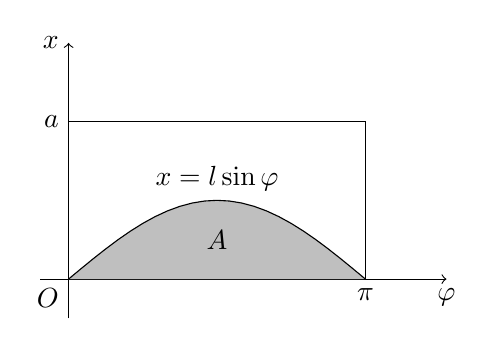
\begin{tikzpicture}[xscale=1.2]
                % 坐标轴
                \draw[->] (-0.3, 0)--(4, 0) node[below]{$\varphi$};
                \draw[->] (0, -0.5)--(0, 3) node[left]{$x$};
                \node at (0, 0) [below left] {$O$};
                % 定义特殊点
                \coordinate (a) at (0, 2);
                \coordinate (p) at (pi, 0);
                % 矩形
                \draw (a) node[left]{$a$} rectangle (p) node[below]{$\pi$};
                % 矩形右上角
                \node at (pi, 2) [below left] {$\varOmega$};
                % 曲线
                \draw[domain=0:pi, fill=lightgray] plot (\x, {sin(\x r)});
                \node at (pi/2, 1) [above] {$x=l \sin \varphi$};
                \node at (pi/2, 1/2) {$A$};
            \end{tikzpicture}
            
            \caption{}
            \label{fig:pufeng:2}
        \end{minipage}
    \end{figure}
\end{solution}

\begin{note}
    \indent 蒲丰投针问题可以用来计算 $\pi$ 的近似值.如果投针 $N$ 次,其中针与平行线相交 $n$ 次,当 $N$ 很大时,以频率 $\dfrac{n}{N}$ 作为概率 $p$ 的近似值,代入式 \eqref{equation:pufeng} 可得
    $$
    \pi = \dfrac{2l}{ap} \approx \dfrac{2lN}{an}
    $$

    设计一个随机试验,使一个事件的概率与某个未知数有关,然后通过重复试验,用频率估计概率,即可求出未知数的近似值.这种方法称为\textbf{随机模拟法},又称为\textbf{蒙特卡罗法}(Monte Carlo method).
\end{note}

\begin{example}[][贝特朗奇论]
    \indent 在一圆内任取一条弦,求该弦的长度超过该圆内接等边三角形的边长的概率.
\end{example}

\begin{solution}

    \textbf{解法一:}由于对称性,可只考察某指定方向的弦,作一条直径垂直于这个方向,只有交直径于 $\dfrac{1}{4}$ 与 $\dfrac{3}{4}$ 之间的弦才能超过内接等边三角形的边长,如图 \ref{fig:贝特朗奇论1} 所示.因此,所求概率为 $\dfrac{1}{2}$.

    \vspace{0.5em}

    \textbf{解法二:}由于对称性,可让弦的一个端点固定,让另一端点在圆周上运动.若在固定端点作切线,则与此切线夹角在 $60^{\circ}$ 与 $120^{\circ}$ 之间的弦才能超过内接等边三角形的边长,如图 \ref{fig:贝特朗奇论2} 所示.因此,所求概率为 $\dfrac{1}{3}$.

    \vspace{0.5em}

    \textbf{解法三:}圆内弦的位置由该弦的中点唯一确定.在圆内作一同心圆,其半径为大圆半径的一半,这个小圆即为大圆内接等边三角形的内接圆.只有大圆上的弦的中点落在小圆内,此弦长才能超过内接等边三角形的边长,如图 \ref{fig:贝特朗奇论3} 所示.因此,所求概率为 $\dfrac{1}{4}$.

    \begin{figure}[H]
        \centering

        \subcaptionbox{\label{fig:贝特朗奇论1}}{
            \centering
            \begin{tikzpicture}[scale=0.7]
                % 定义常量
                \def\r{2} % 半径
                % 定义特殊点
                \coordinate (A) at (0, \r);
                \coordinate (B) at (0, -\r);
                \coordinate (C) at (-0.866*\r, 0.5*\r);
                \coordinate (D) at (0.866*\r, 0.5*\r);
                \coordinate (E) at (-0.9682*\r, 0.25*\r);
                \coordinate (F) at (0.9682*\r, 0.25*\r);
                \coordinate (G) at (0, 0.25*\r); % 垂足
                % 画图
                \draw (0,0) circle (\r); % 圆
                \draw[dashed] (A) -- (B); % 直径
                \draw[dashed] (B) -- (C) -- (D) -- cycle; % 内接等边三角形
                \draw (E) -- (F); % 弦
                \pic[draw=black, -, angle radius=0.2cm] {right angle = F--G--A}; % 垂直记号
            \end{tikzpicture}
        }
        \hspace{1em}
        \subcaptionbox{\label{fig:贝特朗奇论2}}{
            \centering
            \begin{tikzpicture}[scale=0.7]
                % 定义常量
                \def\r{2} % 半径
                % 定义特殊点
                \coordinate (A) at (-1.2*\r, -\r);
                \coordinate (B) at (1.2*\r, -\r);
                \coordinate (C) at (0, -\r);
                \coordinate (D) at (-0.866*\r, 0.5*\r);
                \coordinate (E) at (0.866*\r, 0.5*\r);
                % 画图
                \draw (0,0) circle (\r); % 圆
                \draw[dashed] (A) -- (B); % 切线
                \draw[dashed] (C) -- (D) -- (E) -- cycle; % 内接等边三角形
                \pic["$60^{\circ}$", draw=black, -, angle eccentricity=1.8, angle radius=0.4cm] {angle = D--C--A};
                \pic["$60^{\circ}$", draw=black, -, angle eccentricity=1.6, angle radius=0.5cm] {angle = E--C--D};
                \draw (C) -- (0.6*\r, 0.8*\r); % 弦
            \end{tikzpicture}
        }
        \hspace{1em}
        \subcaptionbox{\label{fig:贝特朗奇论3}}{
            \centering
            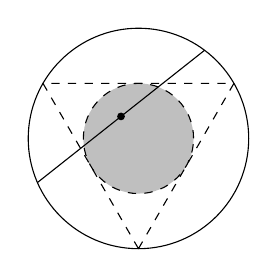
\begin{tikzpicture}[scale=0.7]
                \def\r{2} % 半径
                \draw (0,0) circle (\r); % 圆
                \draw[dashed, fill=lightgray] (0,0) circle (0.5*\r); % 小圆
                \draw[dashed] (0, -\r) -- (-0.866*\r, 0.5*\r) -- (0.866*\r, 0.5*\r) -- cycle; % 内接等边三角形
                \draw (0.6*\r, 0.8*\r) -- (-0.9165*\r, -0.4*\r); % 弦
                \fill (-0.15825*\r, 0.2*\r) circle (2pt); % 弦的中点
            \end{tikzpicture}
        }

        \caption{贝特朗奇论}
    \end{figure}
\end{solution}

\begin{note}
    \indent 同一问题有三种不同答案,这是因为在圆内取弦时规定不够具体,不同的取法导致了不同的样本空间.

    \begin{itemize}
        \item 解法一中假定弦的中点在直径上均匀分布,直径上的点组成样本空间 $\varOmega_1$.
        \item 解法二中假定弦的另一活动端点在圆周上均匀分布,圆周上的点组成样本空间 $\varOmega_2$.
        \item 解法三中假定弦的中点在大圆内均匀分布,大圆内的点组成样本空间 $\varOmega_3$.
    \end{itemize}

    可见,上述三个答案针对的是三个不同的样本空间,它们都是正确的.贝特朗奇论提醒我们,在定义概率时需要明确指出其样本空间.
\end{note}

\section{条件概率}

\subsection{条件概率及其性质}

\begin{definition}[][][def:条件概率]
    \indent 设 $A$ 和 $B$ 是样本空间 $\varOmega$ 中的两个事件,若 $P(B)>0$,则称
    $$
    P(A \mid B) = \dfrac{P(AB)}{P(B)}
    $$
    为``在事件 $B$ 发生的条件下事件 $A$ 发生的概率",简称\textbf{条件概率}(conditional probability).
\end{definition}

\begin{note}
    \indent 条件概率的本质是样本空间的改变.计算 $P(A)$ 时,样本空间为 $\varOmega$;而在事件 $B$ 发生的条件下,所有可能出现的样本点一定在 $B$ 中,因此条件概率 $P(A \mid B)$ 的样本空间为 $B$.

    在定义 \ref{def:条件概率} 中, $B$ 为样本空间, $AB$ 为事件 $A$ 落在样本空间 $B$ 中的部分,因此 $\dfrac{P(AB)}{P(B)}$ 即为条件概率 $P(A \mid B)$.
\end{note}

\begin{property}
    \indent 若 $P(B) > 0$,则有:
    \begin{enumerate}
        \item 非负性: $P(A \mid B) \geqslant 0, A \in \mathcal{F}$.
        \item 规范性: $P(\varOmega \mid B) = 1$.
        \item 可列可加性:若 $A_1, A_2, \cdots, A_n, \cdots$ 两两互斥,则
        $$
        P \left( \bigcup_{i=1}^{\infty} A_i \mid B \right) = \sum_{i=1}^{\infty} P(A_i \mid B)
        $$
    \end{enumerate}
\end{property}

\begin{proof}
    (1) 由定义 \ref{def:条件概率} 得
    $$P(A \mid B) = \dfrac{P(AB)}{P(B)}$$
    而 $P(AB) \geqslant 0, P(B)>0$,因此 $P(A \mid B) \geqslant 0$.

    (2)
    $$
    P(\varOmega \mid B) = \dfrac{P(\varOmega B)}{P(B)} = \dfrac{P(B)}{P(B)} = 1
    $$

    (3)若 $A_1, A_2, \cdots, A_n, \cdots$ 两两互斥,则 $A_1 B, A_2 B, \cdots, A_n B, \cdots$ 也两两互斥,因此
    $$
    \begin{aligned}
        P \left( \bigcup_{i=1}^{\infty} A_i \mid B \right) &= \dfrac{P \left( \left( \displaystyle\bigcup_{i=1}^{\infty} A_i \right) B \right)}{P(B)} \\
        &= \dfrac{P \left( \displaystyle\bigcup_{i=1}^{\infty} (A_i B) \right)}{P(B)} \\
        &= \dfrac{\displaystyle\sum_{i=1}^{\infty} P(A_i B)}{P(B)} \\
        &= \sum_{i=1}^{\infty} \dfrac{P(A_i B)}{P(B)} \\
        &= \sum_{i=1}^{\infty} P(A_i \mid B)
    \end{aligned}
    $$

    \vspace{-2em}
\end{proof}

\begin{note}
    \indent 条件概率满足概率的公理化定义,因此概率的任何性质对条件概率都成立.
\end{note}

\subsection{乘法公式}

\begin{theorem}[][乘法公式]
    \indent 若 $P(B)>0$,则
    \begin{equation} \label{equation:乘法公式}
        P(AB) = P(B) \, P(A \mid B)    
    \end{equation}
    
    若 $P(A_1 A_2 \cdots A_{n-1}) > 0$ 则
    \begin{equation} \label{equation:一般的乘法公式}
        P(A_1 A_2 \cdots A_n) = P(A_1) \, P(A_2 \mid A_1) \, P(A_3 \mid A_1 A_2) \cdots P(A_n \mid A_1 A_2 \cdots A_{n-1})
    \end{equation}
\end{theorem}

\begin{proof}
    根据定义 \ref{def:条件概率},若 $P(B)>0$,则有 $P(A \mid B) = \dfrac{P(AB)}{P(B)}$,整理即可得到式 \eqref{equation:乘法公式}.

    下面证明式 \eqref{equation:一般的乘法公式}.因为
    $$
    P(A_1) \geqslant P(A_1 A_2) \geqslant \cdots \geqslant P(A_1 A_2 \cdots A_{n-1}) > 0
    $$
    所以式 \eqref{equation:一般的乘法公式} 中的条件概率均有意义,按照条件概率的定义展开,得
    $$
    \begin{aligned}
        & P(A_1) \, P(A_2 \mid A_1) \, P(A_3 \mid A_1 A_2) \cdots P(A_n \mid A_1 A_2 \cdots A_{n-1}) \\
        =\ & P(A_1) \cdot \dfrac{P(A_1 A_2)}{P(A_1)} \cdot \dfrac{P(A_1 A_2 A_3)}{P(A_1 A_2)} \cdots \dfrac{P(A_1 A_2 \cdots A_n)}{P(A_1 A_2 \cdots A_{n-1})} \\
        =\ & P(A_1 A_2 \cdots A_n)
    \end{aligned}
    $$
\end{proof}

\begin{note}
    \indent 乘法公式的理解:事件 $A_1 A_2 \cdots A_n$ 的含义是``事件 $A_1, A_2, \cdots, A_n$ 同时发生'',可以将其看作 $A_1, A_2, \cdots, A_n$ 按顺序依次发生. $A_1$ 发生的概率为 $P(A_1)$,在 $A_1$ 发生的条件下 $A_2$ 发生的概率为 $P(A_2 \mid A_1)$,在 $A_1$ 和 $A_2$ 发生的条件下 $A_3$ 发生的概率为 $P(A_3 \mid A_1 A_2)$, ……,以此类推, $P(A_1 A_2 \cdots A_n)$ 即为以上各概率的乘积.
\end{note}

\begin{example}[][波利亚罐子模型]
    \indent 设罐中有 $b$ 个黑球、$r$ 个红球,每次随机取出1个球,取出后将原球放回,再放入 $c$ 个同色球和 $d$ 个异色球.若连续从罐中取出3个球,求其中有2个红球、1个黑球的概率.
\end{example}

\begin{solution}
    设事件 $A$ 为``连续从罐中取出3个球,其中有2个红球、1个黑球", $B_i$ 为``第 $i$ 次取出的是黑球", $R_j$ 为``第 $j$ 次取出的是红球".所求概率 $P(A)$ 与黑球在第几次被取出有关,下面进行分类讨论.

    (1)黑球在第1次被取出:第1次取球时有 $b$ 个黑球、$r$ 个红球,取出的是黑球;第2次取球时有 $b+c$ 个黑球、$r+d$ 个红球,取出的是红球;第3次取球时有 $b+c+d$ 个黑球、$r+d+c$ 个红球,取出的是红球.因此

    $$
    \begin{aligned}
        P(A) &= P(B_1 R_2 R_3) \\
        &= P(B_1) \, P(R_2 \mid B_1) \, P(R_3 \mid B_1 R_2) \\
        &= \dfrac{b}{b+r} \cdot \dfrac{r+d}{b+r+c+d} \cdot \dfrac{r+d+c}{b+r+2c+2d}
    \end{aligned}
    $$

    (2)黑球在第2次被取出:第1次取球时有 $b$ 个黑球、$r$ 个红球,取出的是红球;第2次取球时有 $b+d$ 个黑球、$r+c$ 个红球,取出的是黑球;第3次取球时有 $b+d+c$ 个黑球、$r+c+d$ 个红球,取出的是红球.因此
    $$
    \begin{aligned}
        P(A) &= P(R_1 B_2 R_3) \\
        &= P(R_1) \, P(B_2 \mid R_1) \, P(R_3 \mid R_1 B_2) \\
        &= \dfrac{r}{b+r} \cdot \dfrac{b+d}{b+r+c+d} \cdot \dfrac{r+c+d}{b+r+2c+2d}
    \end{aligned}
    $$

    (3)黑球在第3次被取出:第1次取球时有 $b$ 个黑球、$r$ 个红球,取出的是红球;第2次取球时有 $b+d$ 个黑球、$r+c$ 个红球,取出的是红球;第3次取球时有 $b+2d$ 个黑球、$r+2c$ 个红球,取出的是黑球.因此
    $$
    \begin{aligned}
        P(A) &= P(R_1 R_2 B_3) \\
        &= P(R_1) \, P(R_2 \mid R_1) \, P(B_3 \mid R_1 R_2) \\
        &= \dfrac{r}{b+r} \cdot \dfrac{r+c}{b+r+c+d} \cdot \dfrac{b+2d}{b+r+2c+2d}
    \end{aligned}
    $$
\end{solution}

\begin{note}
    \indent 根据参数 $c,d$ 的不同,波利亚罐子模型可以有各种变化.

    当 $c=-1, d=0$ 时,即为\textbf{不放回抽样}.此时前面的抽取结果会影响后面的抽取,但只要抽取的黑球与红球个数确定,则抽出球的顺序不会影响其概率.
    $$
    \begin{aligned}
        & P(B_1 R_2 R_3) = \dfrac{b}{b+r} \cdot \dfrac{r}{b+r-1} \cdot \dfrac{r-1}{b+r-2} = \dfrac{br(r-1)}{(b+r)(b+r-1)(b+r-2)} \\
        & P(R_1 B_2 R_3) = \dfrac{r}{b+r} \cdot \dfrac{b}{b+r-1} \cdot \dfrac{r-1}{b+r-2} = \dfrac{br(r-1)}{(b+r)(b+r-1)(b+r-2)} \\
        & P(R_1 R_2 B_3) = \dfrac{r}{b+r} \cdot \dfrac{r-1}{b+r-1} \cdot \dfrac{b}{b+r-2} = \dfrac{br(r-1)}{(b+r)(b+r-1)(b+r-2)} \\
    \end{aligned}
    $$

    当 $c=0, d=0$ 时,即为\textbf{放回抽样}.此时前面的抽取结果不会影响后面的抽取.
    $$
    P(B_1 R_2 R_3) = P(R_1 B_2 R_3) = P(R_1 R_2 B_3) = \dfrac{br^2}{(b+r)^3}
    $$

    当 $c>0, d=0$ 时,称为\textbf{传染病模型}.此时,每次取出球后会增加下一次取到同色球的概率,象征每次发现一个传染病患者都会增加再传染的概率.

    在波利亚罐子模型中,只要 $d=0$,上述三个概率都相等.即只要抽取的黑球与红球个数确定,则抽出球的顺序不会影响其概率.
    $$
    P(B_1 R_2 R_3) = P(R_1 B_2 R_3) = P(R_1 R_2 B_3) = \dfrac{br(r+c)}{(b+r)(b+r+c)(b+r+2c)}
    $$

    当 $c=0, d>0$ 时,称为\textbf{安全模型}.此模型可解释为:每当事故发生了(红球被取出),安全工作就抓紧一些,下次再发生事故的概率就会减少;而当事故没有发生时(黑球被取出),安全工作就放松一些,下次发生事故的概率就会增大.此时,上述三个概率不再相等,它们分别为
    $$
    \begin{aligned}
        & P(B_1 R_2 R_3) = \dfrac{b}{b+r} \cdot \dfrac{r+d}{b+r+d} \cdot \dfrac{r+d}{b+r+2d} \\
        & P(R_1 B_2 R_3) = \dfrac{r}{b+r} \cdot \dfrac{b+d}{b+r+d} \cdot \dfrac{r+d}{b+r+2d} \\
        & P(R_1 R_2 B_3) = \dfrac{r}{b+r} \cdot \dfrac{r}{b+r+d} \cdot \dfrac{b+2d}{b+r+2d} \\
    \end{aligned}
    $$
\end{note}

\subsection{全概率公式}

\begin{theorem}[][全概率公式]
    \indent 若事件 $A_1,A_2,\cdots,A_n$ 两两互斥,且 $P(A_i)>0 \ (i=1,2,\cdots,n)$,则对任意事件 $B$,若 $B \subseteq \displaystyle\bigcup_{i=1}^n A_i$,有
    \begin{equation} \label{equation:total}
        P(B) = \sum_{i=1}^n P(A_i) \, P(B \mid A_i)
    \end{equation}
\end{theorem}

\begin{proof}
    因为 $B \subseteq \displaystyle\bigcup_{i=1}^n A_i$,所以
    $$
    B = B \left( \bigcup_{i=1}^n A_i \right) = \bigcup_{i=1}^n(A_i B)
    $$
    由于 $A_1,A_2,\cdots,A_n$ 互斥,所以 $A_1 B, A_2 B, \cdots, A_n B$ 也互斥,由概率的有限可加性得
    $$
    P(B) = P \left( \bigcup_{i=1}^n (A_i B) \right) = \sum_{i=1}^n P(A_i B)
    $$
    由乘法公式得
    $$
    P(B) = \sum_{i=1}^n P(A_i) \, P(B \mid A_i)
    $$
\end{proof}

\begin{note}
    \begin{enumerate}
        \item 全概率公式的最简单形式:若 $0 < P(A) < 1$,则
        $$
        P(B) = P(A) \, P(B \mid A) + P(\overline{A}) \, P(B \mid \overline{A})
        $$
        \item 将条件改成``$A_1, A_2, \cdots, A_n, \cdots$ 两两互斥, $P(A_i)>0 \ (i=1,2,\cdots)$,且 $B \subseteq \displaystyle\bigcup_{i=1}^{\infty} A_i$",全概率公式仍然成立,只需要将式 \eqref{equation:total} 右侧改成可列项之和即可.
        \item $P(A_i)$ 可以看做事件 $A_i$ 对事件 $B$ 的重要程度(权重), $P(A_i) \, P(B \mid A_i)$ 为事件 $A_i$ 对事件 $B$ 的贡献.全概率公式就是将 $A_i \, (i=1,2,\cdots,n)$ 对 $B$ 的贡献加在一起,类似于加权平均.
    \end{enumerate}
\end{note}

\begin{example}[][摸彩模型][example:摸彩模型]
    \indent 设在 $n$ 张彩票中有一张可中奖,求第二个人摸到中奖彩票的概率.
\end{example}

\begin{solution}
    设 $A_i$ 表示事件``第 $i$ 个人摸到中奖彩票", $i=1,2,\cdots,n$.若第一个人摸到中奖彩票,则第二个人不可能再中奖,因此
    $$
    \begin{aligned}
        & P(A_1) = \dfrac{1}{n} \\
        & P(A_2 \mid A_1) = 0
    \end{aligned}
    $$
    若第一个人没有摸到中奖彩票,则第二个人要从剩下的 $n-1$ 张彩票中摸奖,此时有
    $$
    \begin{aligned}
        & P(\overline{A_1}) = \dfrac{n-1}{n} \\
        & P(A_2 \mid \overline{A_1}) = \dfrac{1}{n-1}
    \end{aligned}
    $$
    由全概率公式得
    $$
    \begin{aligned}
        P(A_2) &= P(A_1) \, P(A_2 \mid A_1) + P(\overline{A_1}) \, P(A_2 \mid \overline{A_1}) \\
        &= \dfrac{1}{n} \times 0 + \dfrac{n-1}{n} \cdot \dfrac{1}{n-1} \\
        &= \dfrac{1}{n}
    \end{aligned}
    $$
\end{solution}

\begin{note}
    \indent 例题 \ref{example:摸彩模型} 表明,摸到中奖彩票的机会与先后次序无关.用类似的方法可得
    $$
    P(A_3) = P(A_4) = \cdots = P(A_n) = \dfrac{1}{n}
    $$
    
    如果 $n$ 张彩票中有 $k$ 张可中奖, $k \leqslant n$,则
    $$
    P(A_1) = P(A_2) = \cdots = P(A_n) = \dfrac{k}{n}
    $$
\end{note}

\subsection{贝叶斯公式}

如果事件 $B$ 是由于在两两互斥的事件 $A_1,A_2,\cdots,A_n$ 中某一个发生的情况下而发生的,并且知道各个事件 $A_i$ 发生的概率 $P(A_i)$ 以及在事件 $A_i$ 发生的条件下事件 $B$ 发生的条件概率 $P(B \mid A_i)$,则由全概率公式可得事件 $B$ 发生的概率 $P(B)$.我们把事件 $A_1,A_2,\cdots,A_n$ 看做是导致事件 $B$ 发生的原因, $P(A_i)$ 称为\textbf{先验概率},它反映出各种原因发生的可能性大小.如果在试验中发生了事件 $B$,这一信息有助于探讨事件 $B$ 发生的原因.条件概率 $P(A_i \mid B)$ 称为\textbf{后验概率},它使得我们在试验之后对各种原因发生的可能性大小有进一步的了解.

\begin{theorem}[][贝叶斯公式]
    \indent 对于任意事件 $A,B$,如果 $P(A)>0, P(B)>0$,则
    \begin{equation} \label{equation:贝叶斯}
        P(A \mid B)=\dfrac{P(A) \, P(B \mid A)}{P(B)}
    \end{equation}

    若事件 $A_1,A_2,\cdots,A_n$ 两两互斥,且 $P(A_i)>0 \ (i=1,2,\cdots,n)$,则对任意事件 $B$,如果 $P(B)>0$,且 $B \subseteq \displaystyle\bigcup_{i=1}^n A_i$,有
    \begin{equation} \label{equation:bayes}
        P(A_i \mid B) = \dfrac{P(A_i) \, P(B \mid A_i)}{\displaystyle\sum_{j=1}^n P(A_j) \, P(B \mid A_j)}
    \end{equation}
\end{theorem}

\begin{proof}
    如果 $P(A)>0, P(B)>0$,由乘法公式可得
    $$
    P(AB) = P(B) \, P(A \mid B) = P(A) \, P(B \mid A)
    $$
    由此得
    $$
    P(A \mid B)=\dfrac{P(A) \, P(B \mid A)}{P(B)}
    $$
    式 \eqref{equation:贝叶斯} 得证.

    对于任一事件 $A_i$,有
    $$
    P(A_i \mid B)=\dfrac{P(A_i) \, P(B \mid A_i)}{P(B)}
    $$
    利用全概率公式,得
    $$
    P(A_i \mid B) = \dfrac{P(A_i) \, P(B \mid A_i)}{\displaystyle\sum_{j=1}^n P(A_j) \, P(B \mid A_j)}
    $$
    式 \eqref{equation:bayes} 得证.
\end{proof}

\begin{note}
    \indent $P(A_i) \, P(B \mid A_i)$ 表示事件 $A_i$ 对事件 $B$ 的贡献,贝叶斯公式计算事件 $A_i$ 的贡献在所有贡献中的占比,以此估计事件 $A_i$ 的发生概率.
\end{note}

\section{事件的独立性}

事件的独立性是指一个事件的发生不影响其他事件的发生,也不受其他事件的影响.对于事件 $A$ 与 $B$,当 $P(B) > 0$ 时,条件概率 $P(A \mid B)$ 存在.如果 $P(A \mid B) \not= P(A)$,就意味着事件 $B$ 的发生改变了事件 $A$ 发生的概率,也即事件 $B$ 对事件 $A$ 有某种影响.如果事件 $A$ 与 $B$ 的发生不会相互影响,则有 $P(A \mid B) = P(A)$, 由乘法公式可得
$$
\dfrac{P(AB)}{P(B)} = P(A)
$$
进一步有

\begin{equation} \label{equation:相互独立}
    P(AB) = P(A) \, P(B)
\end{equation}
当 $P(A)=0$ 或 $P(B)=0$ 时,式 \eqref{equation:相互独立} 仍然成立,因此用式 \eqref{equation:相互独立} 作为事件相互独立的定义.

\begin{definition}[][][def:event-independence]
    \indent 对于任意事件 $A,B$,如果 $P(AB) = P(A) \, P(B)$,则称事件 $A$ 与 $B$ \textbf{相互独立}(mutually independent).
\end{definition}

\begin{note}
    \indent 当事件 $A$ 与 $B$ 互斥,且 $P(A) \not= 0, P(B) \not= 0$ 时,事件 $A$ 与 $B$ 一定不相互独立,因为此时 $P(AB) = 0$,而 $P(A) \, P(B) \not= 0$.反之,当事件 $A$ 与 $B$ 相互独立,且 $P(A) \not= 0, P(B) \not= 0$ 时,事件 $A$ 与 $B$ 一定不互斥,因为此时 $P(AB) = P(A) \, P(B) \not= 0$.总之,当两个事件的概率都不为0时,互斥一定不相互独立,相互独立一定不互斥.
\end{note}

\begin{conclusion}
    \indent 若 $P(A)=0$,则事件 $A$ 与任意事件 $B$ 相互独立.
\end{conclusion}

\begin{proof}
    因为 $AB \subseteq A$,由概率的单调性可得 $P(AB) \leqslant P(A) = 0$,又因为 $P(AB) \geqslant 0$,所以 $P(AB) = 0$.进而有
    $$
    P(AB) = P(A) \, P(B) = 0
    $$
    所以 $A$ 与 $B$ 相互独立.
\end{proof}

\begin{conclusion}
    \indent 若 $P(A)=1$,则事件 $A$ 与任意事件 $B$ 相互独立.
\end{conclusion}

\begin{proof}
    因为 $A \subseteq A \cup B$,由概率的单调性可得 $P(A) \leqslant P(A \cup B)$,又因为 $P(A)=1, P(A \cup B) \leqslant 1$,所以 $P(A \cup B) = 1$.用加法公式展开可得
    $$
    P(A \cup B) = P(A) + P(B) - P(AB) = 1 + P(B) - P(AB) = 1
    $$
    整理得
    $$
    P(AB) = P(B) = P(A) \, P(B)
    $$
    所以 $A$ 与 $B$ 相互独立.
\end{proof}

\begin{note}
    \indent 上述结论说明,概率为0的事件与任意事件相互独立,概率为1的事件与任意事件相互独立.同理,不可能事件 $\text{\O}$ 与任意事件相互独立,必然事件 $\varOmega$ 与任意事件相互独立.
\end{note}

\begin{conclusion}
    \indent 对于任意事件 $A,B$,如果 $P(A) > 0$,则 $A$ 与 $B$ 相互独立的充要条件是 $P(B \mid A) = P(B)$;如果 $P(B) > 0$,则 $A$ 与 $B$ 相互独立的充要条件是 $P(A \mid B) = P(A)$.
\end{conclusion}

\begin{conclusion}
    \indent 如果事件 $A$ 与 $B$ 相互独立,则 $A$ 与 $\overline{B}$ 相互独立, $\overline{A}$ 与 $B$ 相互独立, $\overline{A}$ 与 $\overline{B}$ 相互独立.
\end{conclusion}

\begin{proof}
    \vspace{-1em}
    $$
    \begin{aligned}
        P(A \overline{B}) &= P(A-B) \\
        &= P(A) - P(AB) \\
        &= P(A) - P(A) \, P(B)\\
        &= P(A)[1-P(B)]\\
        &= P(A) \, P(\overline{B})
    \end{aligned}
    $$
    因此事件 $A$ 与 $\overline{B}$ 相互独立.

    $$
    \begin{aligned}
        P(\overline{A} B) &= P(B-A) \\
        &= P(B) - P(AB) \\
        &= P(B) - P(A) \, P(B) \\
        &= [1-P(A)] P(B) \\
        &= P(\overline{A}) \, P(B)
    \end{aligned}
    $$
    因此事件 $\overline{A}$ 与 $B$ 相互独立.

    $$
    \begin{aligned}
        P(\overline{A} \cap \overline{B}) &= P(\overline{A \cup B}) \\
        &= 1 - P(A \cup B) \\
        &= 1 - [P(A) + P(B) - P(AB)] \\
        &= 1 - P(A) - P(B) + P(A) \, P(B) \\
        &= [1-P(A)] - P(B) [1-P(A)] \\
        &= [1-P(A)][1-P(B)] \\
        &= P(\overline{A}) \, P(\overline{B})
    \end{aligned}
    $$
    因此事件 $\overline{A}$ 与 $\overline{B}$ 相互独立.
\end{proof}

\begin{definition}[][][def:independent-of-each-other-3]
    \indent 对于任意三个事件 $A,B,C$,如果满足
    \begin{gather*}
        P(AB) = P(A) \, P(B) \\
        P(BC) = P(B) \, P(C) \\
        P(AC) = P(A) \, P(C)
    \end{gather*}
    则称三个事件 $A,B,C$ \textbf{两两相互独立}(pairwise independent).
\end{definition}

\begin{definition}[][][def:independent-3]
    \indent 如果三个事件 $A,B,C$ 两两相互独立,并且有 $P(ABC)=P(A)\,P(B)\,P(C)$,则称三个事件 $A,B,C$ \textbf{相互独立}.
\end{definition}

\begin{note}
    \indent 如果三个事件两两相互独立,不能直接推出这三个事件相互独立.例如:一个均匀的四面体,一面红色,一面黄色,一面蓝色,一面三种颜色都有,抛掷该四面体,设事件 $A=$ ``朝下的面包含红色",事件 $B=$ ``朝下的面包含黄色",事件 $C=$ ``朝下的面包含蓝色",则
    $$
    \begin{aligned}
        & P(A) = P(B) = P(C) = \dfrac{1}{2} \\
        & P(AB) = P(BC) = P(AC) = \dfrac{1}{4} \\
        & P(ABC) = \dfrac{1}{4} \not= P(A) \, P(B) \, P(C)
    \end{aligned}
    $$
    可得事件 $A,B,C$ 两两相互独立,但这三个事件不相互独立.

    当 $P(ABC)=P(A)\,P(B)\,P(C)$ 成立时,不能推出 $A,B,C$ 两两相互独立.例如:设 $\varOmega = \{ \omega_1, \omega_2, \omega_3, \omega_4, \omega_5 \}, P(\{ \omega_1 \}) = \dfrac{1}{64}, P(\{ \omega_2 \}) = P(\{ \omega_3 \}) = P(\{ \omega_4 \}) = \dfrac{15}{64}, P(\{ \omega_5 \}) = \dfrac{18}{64}$,事件 $A = \{ \omega_1, \omega_2 \}, B = \{ \omega_1, \omega_3 \}, C = \{ \omega_1, \omega_4 \}$,则

    $$
    \begin{aligned}
        & P(A) = P(\{ \omega_1 \}) + P(\{ \omega_2 \}) = \dfrac{1}{64} + \dfrac{15}{64} = \dfrac{1}{4} \\
        & P(B) = P(\{ \omega_1 \}) + P(\{ \omega_3 \}) = \dfrac{1}{64} + \dfrac{15}{64} = \dfrac{1}{4} \\
        & P(C) = P(\{ \omega_1 \}) + P(\{ \omega_4 \}) = \dfrac{1}{64} + \dfrac{15}{64} = \dfrac{1}{4} \\
        & P(AB) = P(\{ \omega_1 \}) = \dfrac{1}{64} \\
        & P(ABC) = P(\{ \omega_1 \}) = \dfrac{1}{64} \\
    \end{aligned}
    $$
    此时有 $P(ABC)=P(A)\,P(B)\,P(C)$,但 $P(AB) \not= P(A)\,P(B)$, $A,B,C$ 不两两相互独立.
\end{note}

\begin{conclusion}
    \indent 若 $A,B,C$ 相互独立,则 $A \cup B$ 与 $C$ 相互独立, $AB$ 与 $C$ 相互独立, $A-B$ 与 $C$ 相互独立.
\end{conclusion}

\begin{proof}
    $$
    \begin{aligned}
        P((A \cup B) C) &= P(AC \cup BC) \\
        &= P(AC) + P(BC) - P(ABC) \\
        &= P(A) P(C) + P(B) P(C) - P(A) P(B) P(C) \\
        &= [P(A) + P(B) - P(A) P(B)] P(C) \\
        &= P(A \cup B) P(C)
    \end{aligned}
    $$
    所以 $A \cup B$ 与 $C$ 相互独立.

    $$
    P((AB)C) = P(A) P(B) P(C) = P(AB) P(C)
    $$
    所以 $AB$ 与 $C$ 相互独立.

    $$
    \begin{aligned}
        P((A-B)C) &= P(A \overline{B} C) \\
        &= P(AC-B) \\
        &= P(AC) - P(ABC) \\
        &= P(A) P(C) - P(AB) P(C) \\
        &= [P(A) - P(AB)] P(C) \\
        &= P(A-B) P(C)
    \end{aligned}
    $$
    所以 $A-B$ 与 $C$ 相互独立.
\end{proof}

\begin{note}
    \indent 如果事件 $A,B,C$ 只有两两相互独立,则不能证明 $A \cup B$ 与 $C$ 相互独立、$AB$ 与 $C$ 相互独立、$A-B$ 与 $C$ 相互独立.
\end{note}

\begin{definition}[][][def:independent-more]
    \indent 对于任意 $n$ 个事件 $A_1,A_2,\cdots,A_n$ ,如果其中任意 $k\,(2\leqslant k\leqslant n)$ 个事件 $A_{i_1},A_{i_2},\cdots,A_{i_k}$ 都满足等式
    $$
    P(A_{i_1} A_{i_2} \cdots A_{i_k}) = P(A_{i_1}) \, P(A_{i_2}) \cdots P(A_{i_k})
    $$
    则称这 $n$ 个事件 $A_1,A_2,\cdots,A_n$ \textbf{相互独立}.
\end{definition}

\begin{conclusion}
    \indent 若 $n\, (n \geqslant 2)$ 个事件相互独立,则其中任意 $k\, (2 \leqslant k \leqslant n)$ 个事件相互独立.将其中任意 $k$ 个事件换成对立事件,所得诸事件仍然相互独立.
\end{conclusion}

\section{伯努利概型}

\begin{definition}
    \indent 设有两个试验 $E_1$ 和 $E_2$,假如试验 $E_1$ 的任一结果(事件)与试验 $E_2$ 的任一结果(事件)都是相互独立的事件,则称这两个试验相互独立.
\end{definition}

\begin{definition}
    \indent 如果试验 $E_1$ 的任一结果、试验 $E_2$ 的任一结果、……、试验 $E_n$ 的任一结果都是相互独立的事件,则称试验 $E_1, E_2, \cdots, E_n$ 相互独立.如果这 $n$ 个独立试验是相同的,则称其为 $n$ \textbf{重独立重复试验}(repeated indepentent trials).
\end{definition}

\begin{definition}
    \indent 如果在 $n$ 重独立重复试验中,每次试验的可能结果只有两个($A$ 或 $\overline{A}$),则称这种试验为 $n$ \textbf{重伯努利试验},简称为\textbf{伯努利试验}(Bernoulli trial),也称为\textbf{伯努利概型}(Bernoulli probability model).
\end{definition}

$n$ 重伯努利试验的基本事件可记为 $\omega=\omega_1 \omega_2 \cdots \omega_n$,其中 $\omega_i\,(1\leqslant i\leqslant n)$ 为 $A$ 或者为 $\overline{A}$,即 $\omega$ 是从 $A$ 及 $\overline{A}$ 中每次取 1 个,独立地重复取 $n$ 次的一种排列,共有 $2^n$ 个基本事件.

设 $P(A)=p, P(\overline{A}) = 1-p$,其中 $0<p<1$.如果 $\omega$ 中有 $k$ 个 $A$,则必有 $n-k$ 个 $\overline{A}$,由独立性可得这一基本事件的概率为 $p^k (1-p)^{n-k}$.

由于在 $2^n$ 个基本事件中共有 $\mathrm{C}_n^k$ 个含 $k$ 个 $A$ 及 $n-k$ 个 $\overline{A}$,因此在 $n$ 重伯努利试验中,事件 $A$ 恰好发生 $k$ 次的概率 $P_n(k)$ 为
\begin{gather} \label{equation:binomial}
    P_n(k)=\mathrm{C}_n^k p^k (1-p)^{n-k}, \ k=0,1,2,\cdots,n
\end{gather}

由二项式定理可得
$$
\sum_{k=0}^n P_n(k) = \sum_{k=0}^n \mathrm{C}_n^k p^k (1-p)^{n-k} = [p+(1-p)]^n = 1
$$
由此可见, $\mathrm{C}_n^k p^k (1-p)^{n-k}$ 是二项展开式中的一项,因此式 \eqref{equation:binomial} 又称为\textbf{二项概率公式}(binomial distribution formula).